\hsection{Text Strings}%
\label{sec:str}%
%
The fourth important datatype in \python\ are text strings.
Text strings are sequences of characters of an arbitrary length.
In \python, they are represented by the datatype \pythonilIdx{str}.
Indeed, we have already used it before, even in our very first example program back that simply printed \pythonil{"Hello World"} in \cref{lst:very_first_program} in \cref{sec:ourFirstProgram}.
\pythonil{"Hello World"} is such a text string.%
%
\hsection{Basic String Operations}%
%
\begin{figure}%
\centering%
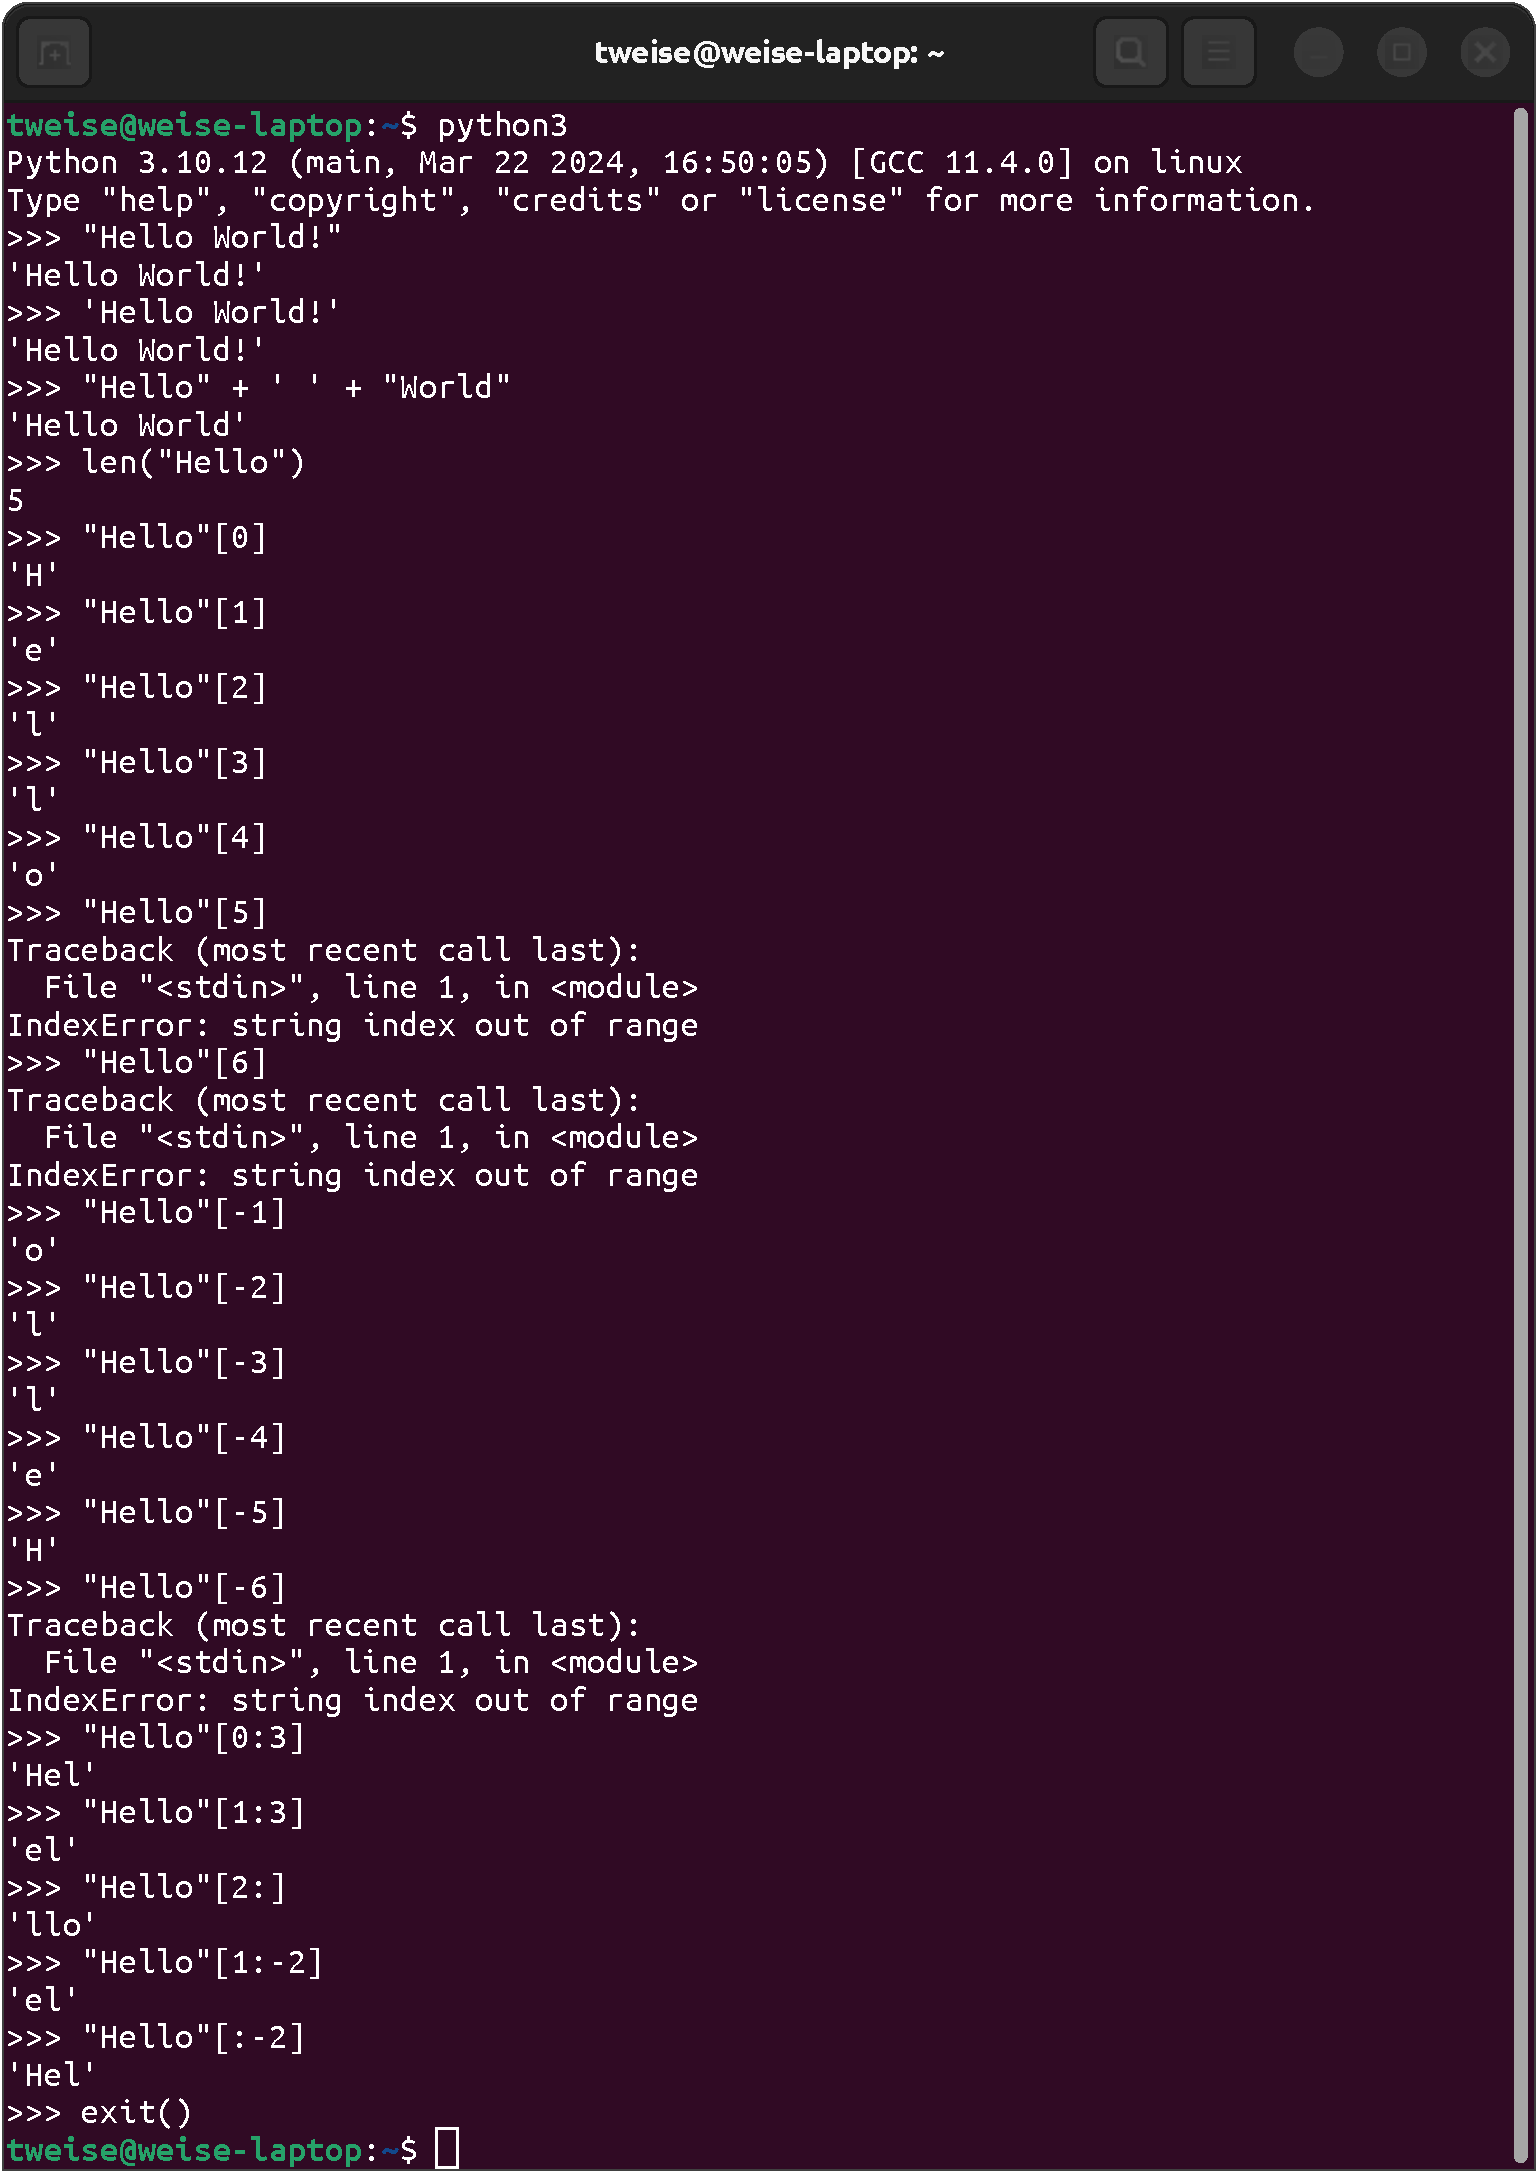
\includegraphics[width=0.8\linewidth]{\currentDir/strIndexing}%
\caption{Specifying string literals and indexing its characters.}%
\label{fig:strIndexing}%
\end{figure}%
%
As \cref{fig:strIndexing} shows, there are two basic ways to specify a text string literal\pythonIdx{str!literal}:
Either enclosed by double quotes, e.g., \pythonil{"Hello World!"}\pythonIdx{\textquotedbl} or enclosed by single quotes, e.g., \pythonil{'Hello World!'}\pythonIdx{\textquotesingle}.
The double-quote variant is usually preferred and we should always use it in our programs.
The quotation marks are only used to delimit the strings, i.e., to tell \python\ where the string begins or ends.
They are not themselves part of the string.

One basic operation is string concatenation\pythonIdx{str!concatenation}\pythonIdx{str!+}\pythonIdx{+}:
\pythonil{"Hello" + ' ' + "World"}\pythonIdx{\textquotedbl}\pythonIdx{\textquotesingle} concatenates the three strings \pythonil{"Hello"}, \pythonil{" "}, and \pythonil{"World"}.
The result is \pythonil{"Hello World"}\pythonIdx{\textquotedbl}.
Notice how the singe space character string is needed, because \pythonil{"Hello" + "World"} would just yield \pythonil{"HelloWorld"}.

Strings are different from the other datatypes we have seen so far.
They are \emph{sequences}\pythonIdx{Sequence}, meaning that they are linear arrays composed of elements.
These elements are the single characters, which correspond to letters, numbers, punctuation marks, white space, etc.

One basic set of things that we can do with strings is to extract these single characters.
First, we need to know the length of a string.
For this purpose, we can invoke the \pythonilIdx{len}\pythonIdx{str!len}\pythonIdx{str!length} function:
\pythonil{len("Hello")} is \pythonil{5}, because there are five characters in \inQuotes{Hello}.
\pythonil{len("Hello World!")} would give us \pythonil{12}, because \pythonil{"Hello"} has five characters, \pythonil{"World!"} has six characters (the \pythonil{"!"} does count!) and there is the single space character in the middle, so $5+6+1=12$.

Knowing the length\pythonIdx{str!length} of a string, we can now safely access its single characters.
These characters are obtained using the square brackets \pythonil{[]}\pythonIdx{str![]}\pythonIdx{[}\pythonIdx{]} with the character index inbetween.
The character indexes start at~0.
Therefore, \pythonil{"Hello"[0]}\pythonIdx{str![]}\pythonIdx{[}\pythonIdx{]} returns the first character of \pythonil{"Hello"} as a \pythonilIdx{str}, which is \pythonil{"H"}\pythonIdx{\textquotedbl}.
\pythonil{"Hello"[1]} returns the second character, which is \pythonil{"e"}.
\pythonil{"Hello"[2]} returns the third character, which is \pythonil{"l"}.
\pythonil{"Hello"[3]}\pythonIdx{str![]}\pythonIdx{[}\pythonIdx{]} gives us the second \pythonil{"l"}.
Finally, \pythonil{"Hello"[4]} gives us the fifth and last character, namely \pythonil{"o"}\pythonIdx{\textquotedbl}.
If we would try to access a character outside of the valid range of the string, say \pythonil{"Hello"[5]}, this results in an \pythonilIdx{IndexError}.
We learn later what errors are and how to handle them -- for now, it is sufficient to know that they will stop your program.
And rightly so, because \pythonil{"Hello"}\pythonIdx{\textquotedbl} has only five characters and accessing the sixth one is not possible and would have an undefined result.

Negative indices, however, are permitted:
The index \pythonil{-1} just means \inQuotes{last character}, so \pythonil{"Hello"[-1]} yields the string \pythonil{"o"}.
The index \pythonil{-2} then refers to the \inQuotes{second-to-last character}, so \pythonil{"Hello"[-2]} gives us \pythonil{"l"}.
The third character from the end, accessed via index \pythonil{-3}, is again \pythonil{"l"}.
\pythonil{"Hello"[-4]} gives us \pythonil{"e"} and \pythonil{"Hello"[-5]} gives us \pythonil{"H"}.
Of course, using a negative index that would bring us out of the string's valid range, such as \pythonil{-6}, again yields an \pythonilIdx{IndexError}.

We can also obtain whole substrings by using index ranges, where the inclusive starting index and the \emph{exclusive} end index are separated by a~\pythonilIdx{:}.
In other words, applying the index \pythonil{[a:b]} to a string results in all characters in the index range from \pythonil{a} to \pythonil{b - 1}.
\pythonil{"Hello"[0:3]} yields a string composed of the characters at positions~0, 1, and~2 inside \pythonil{"Hello"}, i.e., \pythonil{"Hel"}.
The end index is always excluded, so the character at index~3 is not part of the result.
If we do \pythonil{"Hello"[1:3]}, we get \pythonil{"He"}, because only the characters at indices~1 and~2 are included.
If we do not specify an end index, then everything starting at the start index until the end of the string is included.
This means that \pythonil{"Hello"[2:]} will return all the text starting at index~2, which is \pythonil{"llo"}.
We can also use negative indices, if we want.
Therefore, \pythonil{"Hello"[1:-2]} yields \pythonil{"el"}
Finally, we can also omit the start index, in which case everything until right before the end index is returned.
Therefore, \pythonil{"Hello"[:-2]} will return everything from the beginning of the string until right before the second-to-last character.
This gives us \pythonil{"Hel"}.

\begin{figure}%
\centering%
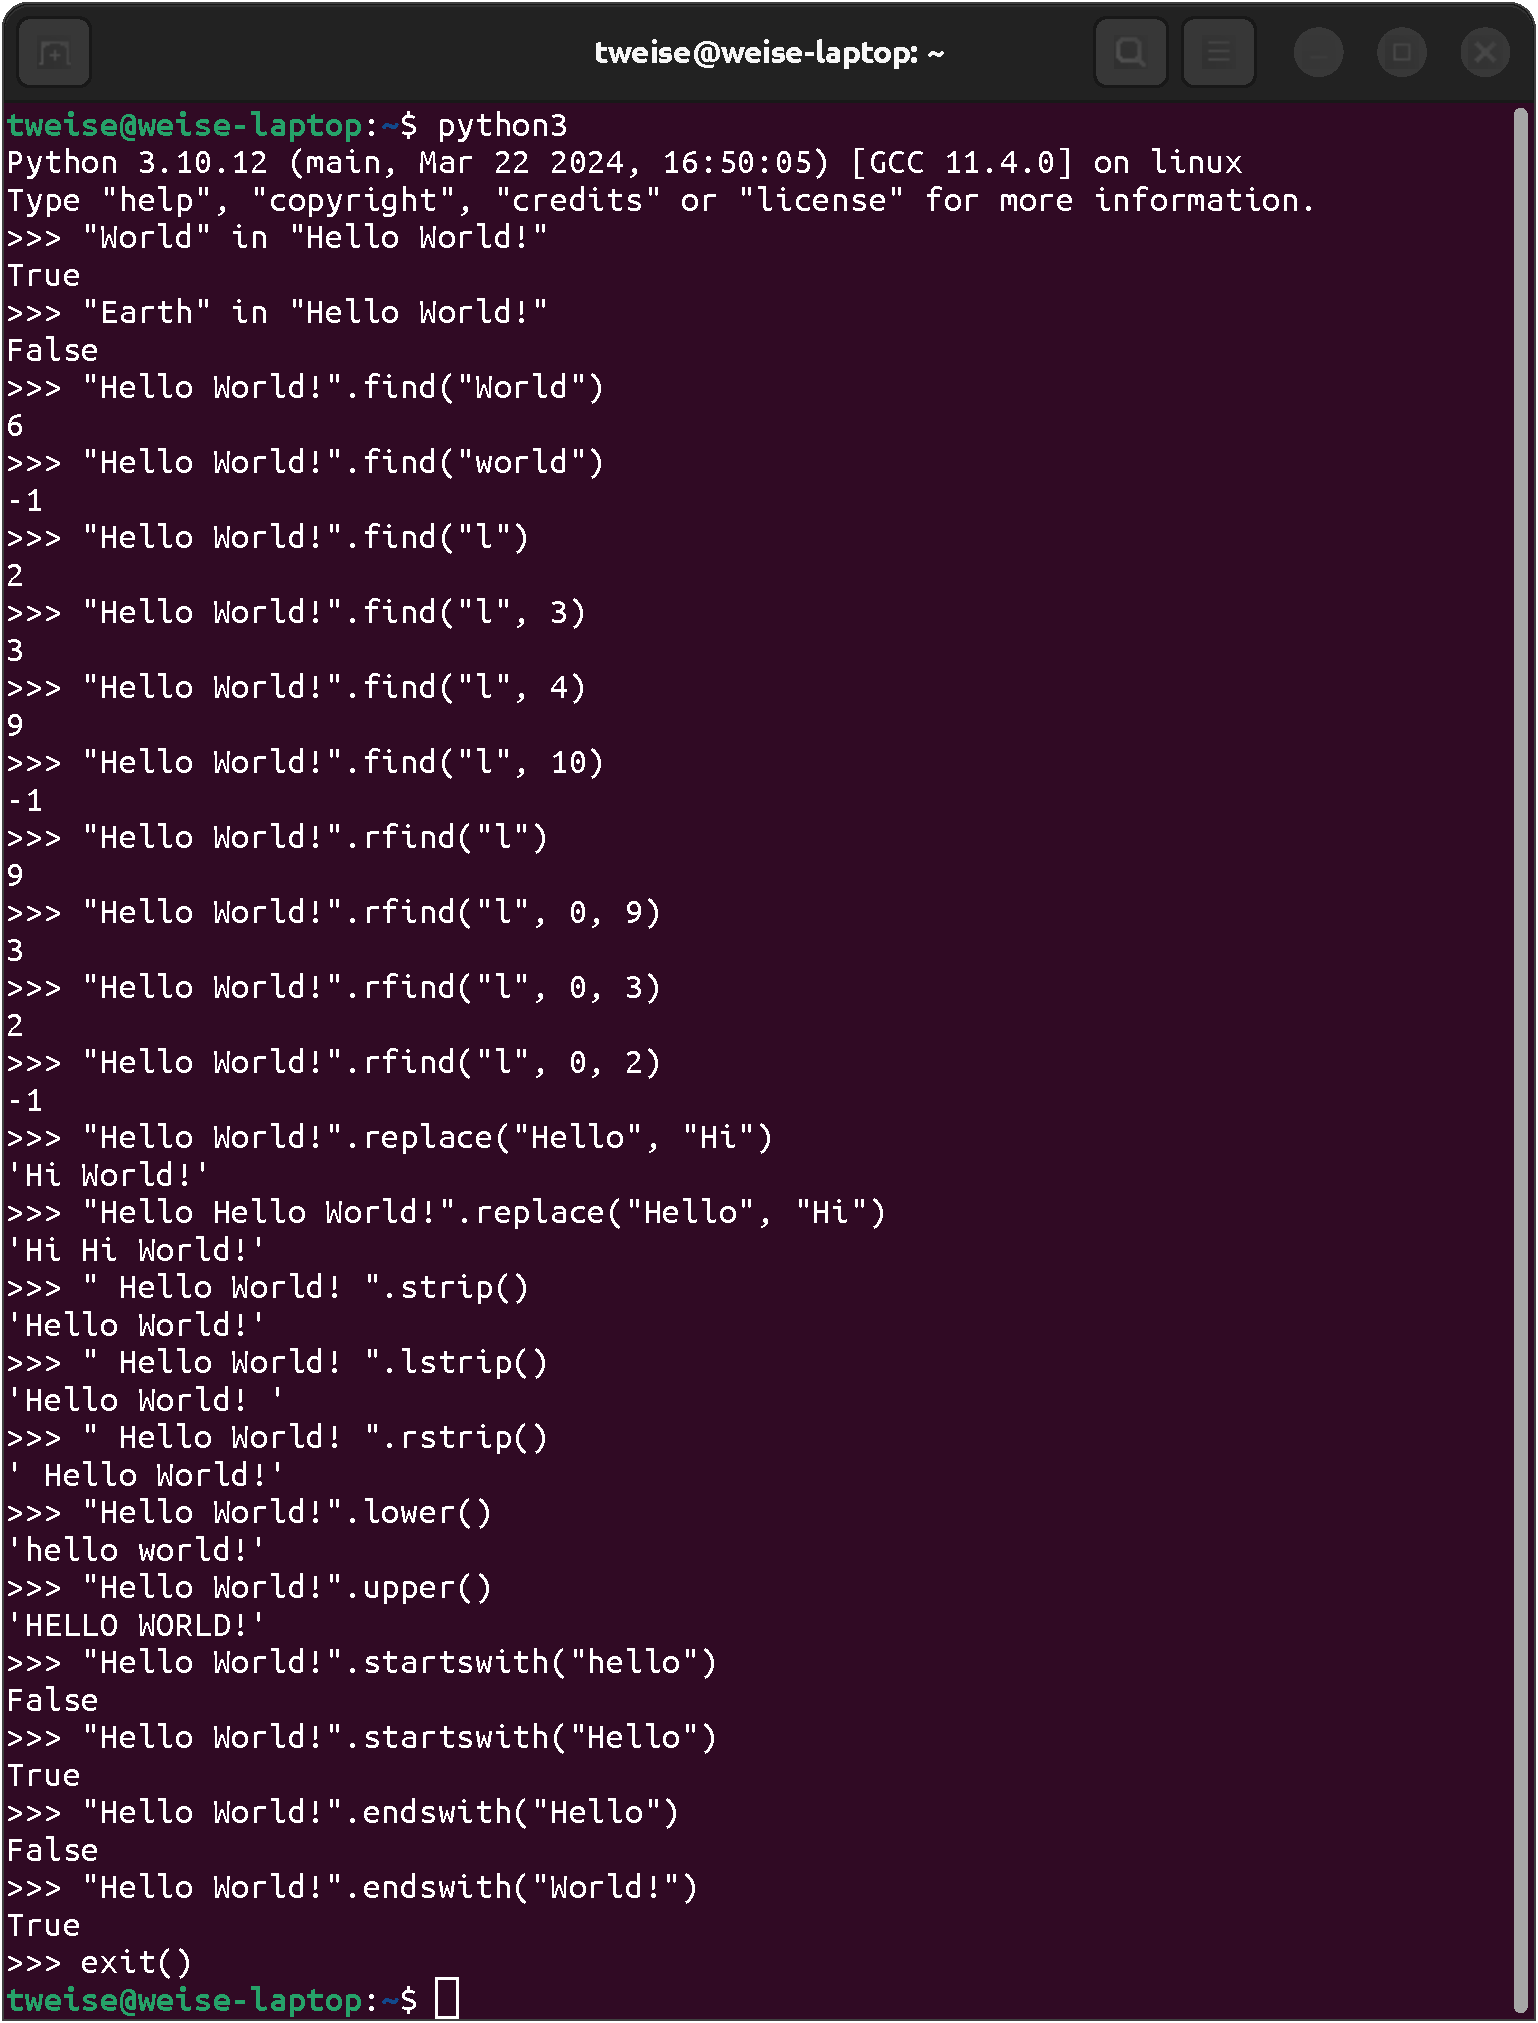
\includegraphics[width=0.8\linewidth]{\currentDir/strBasicOps}%
\caption{Some more basic string operations.}%
\label{fig:strBasicOps}%
\end{figure}%

Besides concatenating and extracting substrings, the \pythonilIdx{str} datatype supports many other operations.
Here, we can just discuss the few most commonly used ones.

There are several ways to check whether one string is contained in another one.
The first method is to use the \pythonilIdx{in} keyword.
As \cref{fig:strBasicOps} shows, \pythonil{"World" in "Hello World!"} yields \pythonilIdx{True}, as it checks whether \pythonil{"World"} is contained in \pythonil{"Hello World!"}, which is indeed the case.
\pythonil{"Earth" in "Hello World!"} is \pythonilIdx{False}, because \pythonil{"Earth"} is not contained in \pythonil{"Hello World!"}.

Often, however, we do not just want to know whether a string is contained in another one, but also \emph{where} it is contained.
For this, the \pythonilIdx{find} method exists.
\pythonil{"Hello World!".find("World")} tries to find the position of \pythonil{"World"} inside \pythonil{"Hello World!"}.
It returns \pythonil{6}, because the \inQuotes{W} of \inQuotes{World} is the seventh character in this string and the indices are zero-based.
Trying to find the \pythonil{"world"} in \pythonil{"Hello World!"} yields~\pythonil{-1}, however.
\pythonil{-1} means that the string cannot be found.
We learn that string operations are case-sensitive\pythonIdx{str!case-sensitive}:
\pythonil{"World" != "world"} would be \pythonilIdx{True}.
We also learn that we need to be careful not to use the result of \pythonilIdx{find} as index in a string directly before checking that it is \pythonil{>= 0}!
As you have learned, \pythonil{-1} is a perfectly fine index into a string, even though it means that the string we tried to find was not found.

Sometimes, the text we are looking for is contained multiple times in a given string.
For example, \pythonil{"Hello World!".find("l")} returns~\pythonil{2}, because \inQuotes{l} is the third character in the string.
However, it is also the fourth character in the string.
\pythonilIdx{find} accepts an optional second parameter, namely the starting index where the search should begin.
\pythonil{"Hello World!".find("l", 3)} begins to search for \pythonil{"l"} inside \pythonil{"Hello World!"} starting at index~3.
Right at that index, the second~\inQuotes{l} is found, so that \pythonil{3} is also returned.
If we search for another~\inQuotes{l} after that, we would do \pythonil{"Hello World!".find("l", 4)}, which returns index~9, identifying the~\inQuotes{l} in~\inQuotes{World}.
After that, no more~\inQuotes{l} can be found in the string, so \pythonil{"Hello World!".find("l", 10)} results in a~\pythonil{-1}.%
%
\begin{sloppypar}%
While \pythonilIdx{find} returns the first occurrence of a string in the supplied range, we sometimes want the last occurrence instead.
If we want to search from the end of the string, we use \pythonilIdx{rfind}.
\pythonil{"Hello World!".rfind("l")} gives us~\pythonil{9} directly.
If we want to search for the~\inQuotes{l} before that one, we need to supply an inclusive starting and exclusive ending index of the range to be searched.
\pythonil{"Hello World!".rfind("l", 0, 9)} searches for any~\inQuotes{l} from index~8 down to~0 and thus returns~\pythonil{3}.
\pythonil{"Hello World!".rfind("l", 0, 3)} gives us~\pythonil{2} and since there is no~\inQuotes{l} before that, \pythonil{"Hello World!".rfind("l", 0, 2)} yields~\pythonil{-1}.
\end{sloppypar}%
%
\begin{sloppypar}%
Another common operation is to replace substrings with something else.
\pythonil{"Hello World!".replace("Hello", "Hi")}\pythonIdx{replace} replaces all occurrences of \inQuotes{"Hello"} in \inQuotes{Hello World} with \inQuotes{Hi}.
The result is \pythonil{"Hi World!"} and \pythonil{"Hello Hello World!".replace("Hello", "Hi")} becomes \pythonil{"Hi Hi World!"}.
\end{sloppypar}%
%
\begin{sloppypar}%
Often, we want to remove all leading or trailing whitespace characters from a string.
The \pythonilIdx{strip} function does this for us:
\pythonil{" Hello World! ".strip()} returns \pythonil{"Hello World!".strip()}, i.e., the same string, but with the leading and trailing space removed.
If we only want to remove the spaces on the left-hand side, we use \pythonilIdx{lstrip} and if we only want to remove those on the right-hand side, we use \pythonilIdx{rstrip} instead.
Therefore, \pythonil{" Hello World! ".lstrip()} yields \pythonil{"Hello World! "} and \pythonil{" Hello World! ".rstrip()} gives us \pythonil{" Hello World!"}.
\end{sloppypar}%
%
In alphabet-based languages, we usually can distinguish between uppercase\pythonIdx{str!uppercase} characters, such as \inQuotes{H} and \inQuotes{W}, and lowercase\pythonIdx{str!lowercase}, such as \inQuotes{e}, \inQuotes{l}, and~\inQuotes{o}.
The method \pythonilIdx{lower} transforms all characters in a string to lowercase and \pythonilIdx{upper} translates them to uppercase instead.
Thus \pythonil{"Hello World!".lower()} returns \pythonil{hello world!} whereas \pythonil{"Hello World!".upper()} yields \pythonil{"HELLO WORLD!"}.

As final functions, we can check whether a string begins or ends with another, we can use \pythonilIdx{startswith} and \pythonilIdx{endswith}, respectively.
\pythonil{"Hello World!".startswith("hello")} is \pythonilIdx{False} whereas \pythonil{"Hello World!".startswith("Hello")} is \pythonilIdx{True}.
\pythonil{"Hello World!".endswith("Hello")} is \pythonilIdx{False}, too, but \pythonil{"Hello World!".endswith("World!")} is \pythonilIdx{True}.

Of course, these were just a small selection of the many string operations available in \python.
You can find more in the \href{https://docs.python.org/3/library/stdtypes.html\#textseq}{official documentation}~\cite{PSF2024TSTS}.%
\endhsection%
%
\endhsection%
%
